\chapter{The search for standard model~\tttt production in \runtwo at $\sqrt{s} =$~13~TeV \label{c:Run2}}


\section{Introduction}
In this chapter, an analysis of the full 2015 CMS data set of proton-proton collisions at $\sqrt{s} =$~13~TeV with 2.6~\fbinv of data is presented where the standard model production of four top quarks (\tttt) is sought. SM \tttt production has a cross section of $\sigmattttSM \approx 0.2$ fb at NLO with NNLO corrections~\cite{Barger201070,Bevilacqua2012}. 

All sections apart from X are the authors personal contribution to the analysis.

\section{Data and Simulation}
\label{sec:datasimulation13}
This analysis uses data from proton-proton collision at the CMS experiment in 2012 at $\sqrt{s}=13$~TeV.
Data were collected using a trigger based on the presence of at least one muon (electron) candidate with $\pt > $~18~(23)~GeV for the muon (electron) channel and corresponds to an integrated luminosity of 2.6~\fbinv .
% The full 2012 SingleElectron dataset is used for the electron channel, which requires an electron candidate with $\pt > $ 27 GeV and corresponds to an integrated luminosity of 19.7 \fbinv.
The signal SM \tttt Monte Carlo (MC) samples and the background MC samples are given in table~\ref{tab:datasets_sim_13tev}, along with the MC generator used to produce these samples, the order at which they were produced and the number of events produced. MC samples were produced for the hadronisation scale systematic, which can be found in table~\ref{tab:datasets_sys_13tev}. In this analysis the ME scale and PS scale are treated as separate uncertainties.

\begin{table}[ht!]
% \tiny
\centering
\begin{tabular}{| l | l | l | p{2cm} |}
 \hline 
 Dataset & Events & Generator & Order \\
\hline
\tttt & 960K & \MADGRAPH\aMCATNLO & NLO \\
\hline
\ttbar &97M & \POWHEG  & NLO \\
\hline
WJetsToLNu & 47M & \MLM & NLO \\
\hline
Tbar\_tW-channel & 1M & \POWHEG & NLO\\
\hline
T\_tW-channel & 1M & \POWHEG & NLO \\
\hline
DYJetsToLL & 9M & \MLM & NLO \\
\hline
TTZJets  & 400K & \MADGRAPH\aMCATNLO & NLO \\
\hline
TTWJets\ & 250K & \MADGRAPH\aMCATNLO & NLO \\
\hline
TTH\_HToBB & 4M & \POWHEG & NLO \\
% \hline
% ZZ & 10M & \PYTHIA 6 & O \\
% \hline
% WZ &10M & \PYTHIA 6 & O \\
% \hline
% WW &10M & \PYTHIA 6 & O \\
\hline
\end{tabular}
 \caption{Dataset name, total number of events, MC generator and order of the simulated samples. \PYTHIA~8 is used to hadronise all samples in this table.}
  \label{tab:datasets_sim_13tev}
  \end{table}


\begin{table}[ht!]
% \tiny
\centering
\begin{tabular}{| l | l | l | p{2cm} |}
 \hline 
 Dataset & Events & Generator & Order \\
\hline
TTJets\_scaledown & 10M  & \POWHEG & NLO \\
\hline
TTJets\_scaleup & 10M  & \POWHEG & NLO \\
\hline
TTJets & 5M & \MLM & NLO  \\
\hline
TTJets & 5M & \MADGRAPH\aMCATNLO & NLO \\
\hline
\end{tabular}
 \caption{Dataset name, total number of events, MC generator and order of the simulated systematic samples. \PYTHIA~8 is used to hadronise all samples in this table.}
  \label{tab:datasets_sys_13tev}
\end{table}

\section{Baseline Event Selection}
\label{sec:baseline13}
The set of criteria applied to the reconstructed objects in events which are triggered by the single muon or single electron triggers in order to select \tttt events and suppress background events is detailed below.

For the muon channel these are:
\begin{itemize}
\setlength\itemsep{0em}
\item Exactly one tight muon
\item Exactly zero additional loose muons
\item Exactly zero loose electrons
\item At least 6 jets with $\pt >$ 30 \GeV
\item At least 2 CSVM tagged b-jets
\end{itemize}
For the electron channel these are:
\begin{itemize}
\itemsep0em 
\item Exactly one tight electron
\item Exactly zero additional loose electrons
\item Exactly zero loose muons
\item At least 6 jets with $\pt >$ 30 \GeV
\item At least 2 CSVM tagged b-jets
\end{itemize}

\section{Corrections to the simulation}
\label{sec:Calibrations13}
All corrections are described in section~\ref{sec:Calibrations}. The PU corrections are applied, producing a good agreement in the distribution of the number of vertices as seen in Fig.~\ref{fig:PUReWeight13}. Muon scale factors~\cite{muonSFtwiki} and electron scale factors~\cite{electronSFtwiki} are applied. By comparing the efficiencies in data with the efficiencies in simulation, a value was obtained of $1.0001\pm0.0001$ for the electron trigger scale factor which was taken to be 1 in the analysis. The method in~\ref{subsec:method2btag} was used to derive the b tagging scale factors.


\begin{figure}[h!]
\begin{center}
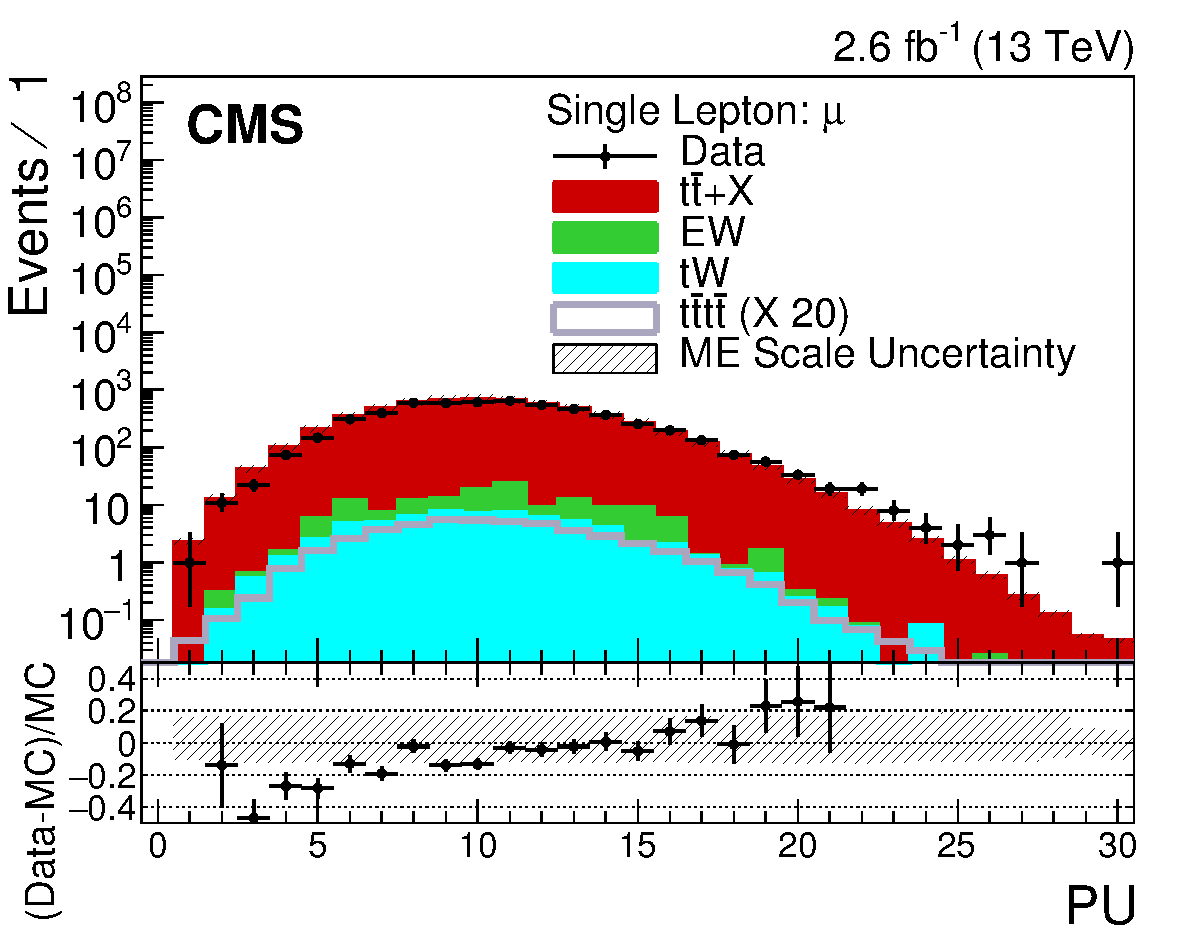
\includegraphics[width=0.67\textwidth]{images/Run2/PU_StackLogY.pdf}
\end{center}
\caption{The number of primary vertices for data and simulation after re-weighting for mu + jets.}
\label{fig:PUReWeight13}
\end{figure} 

The jet multiplicity modelling from section~\ref{subsec:alphaS} was applied. It can be seen from Figs.~\ref{fig:withAlpha} and~\ref{fig:withoutAlpha} that the jet multiplicity modelling is greatly improved by applying this correction.

\begin{figure}[ht!]
    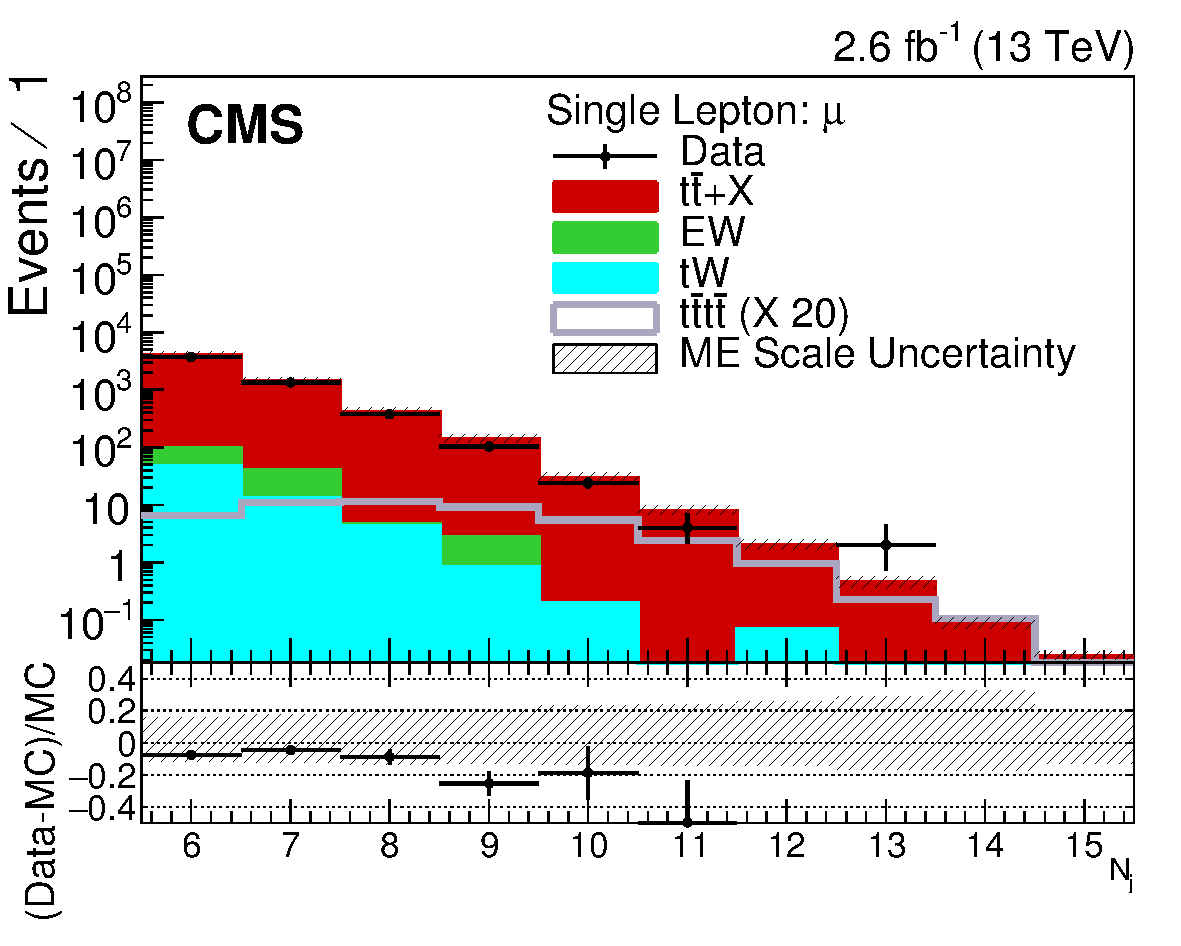
\includegraphics[width=0.48\textwidth]{images/Run2/nJets_StackLogY.pdf}
    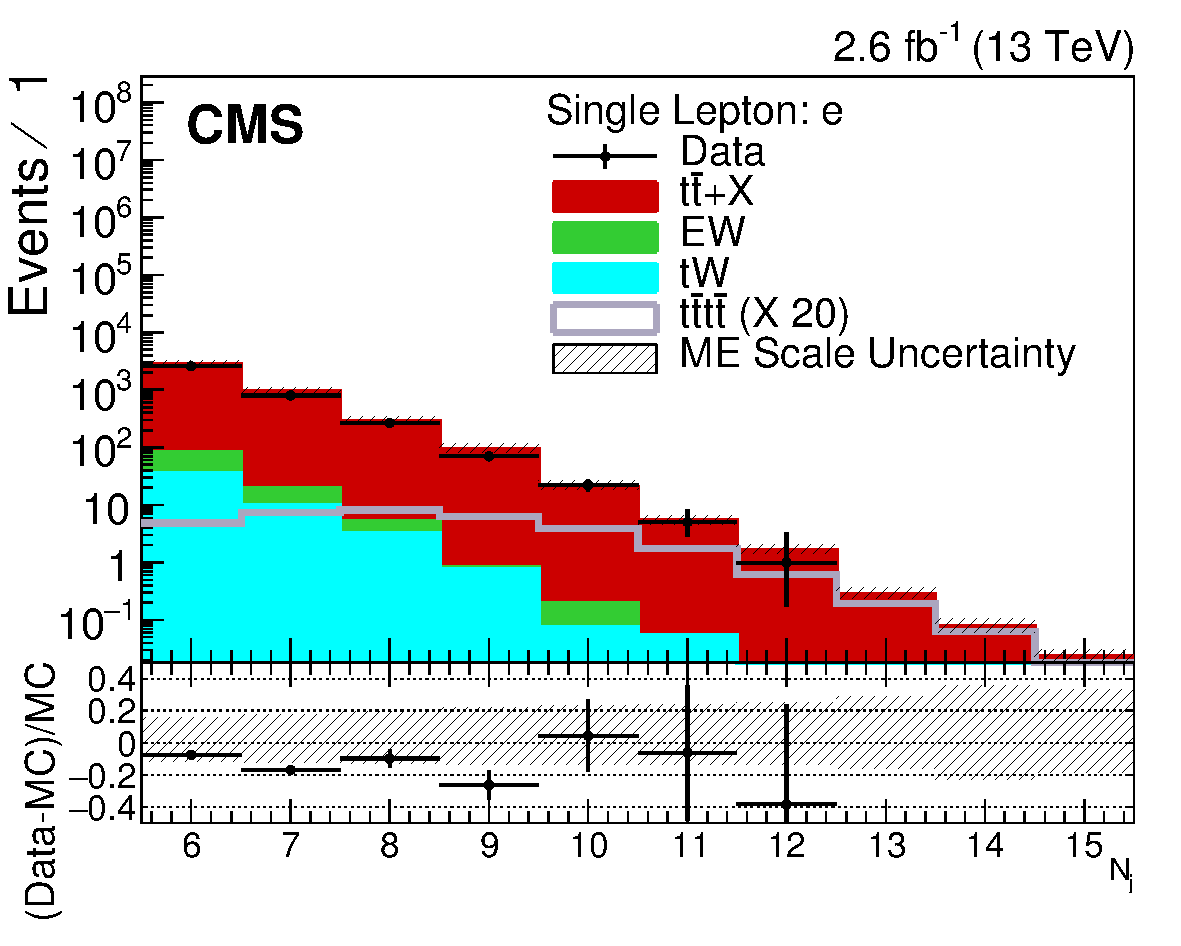
\includegraphics[width=0.48\textwidth]{images/Run2/nJets_StackLogY_e.pdf}
    \caption{The \njets distributions for data and simulation in the $\mu$ + jets channel (left) and $e$ + jets channel (left) with jet multiplicity modelling scale factors applied.}
    \label{fig:withAlpha}
\end{figure}

\begin{figure}[ht!]
    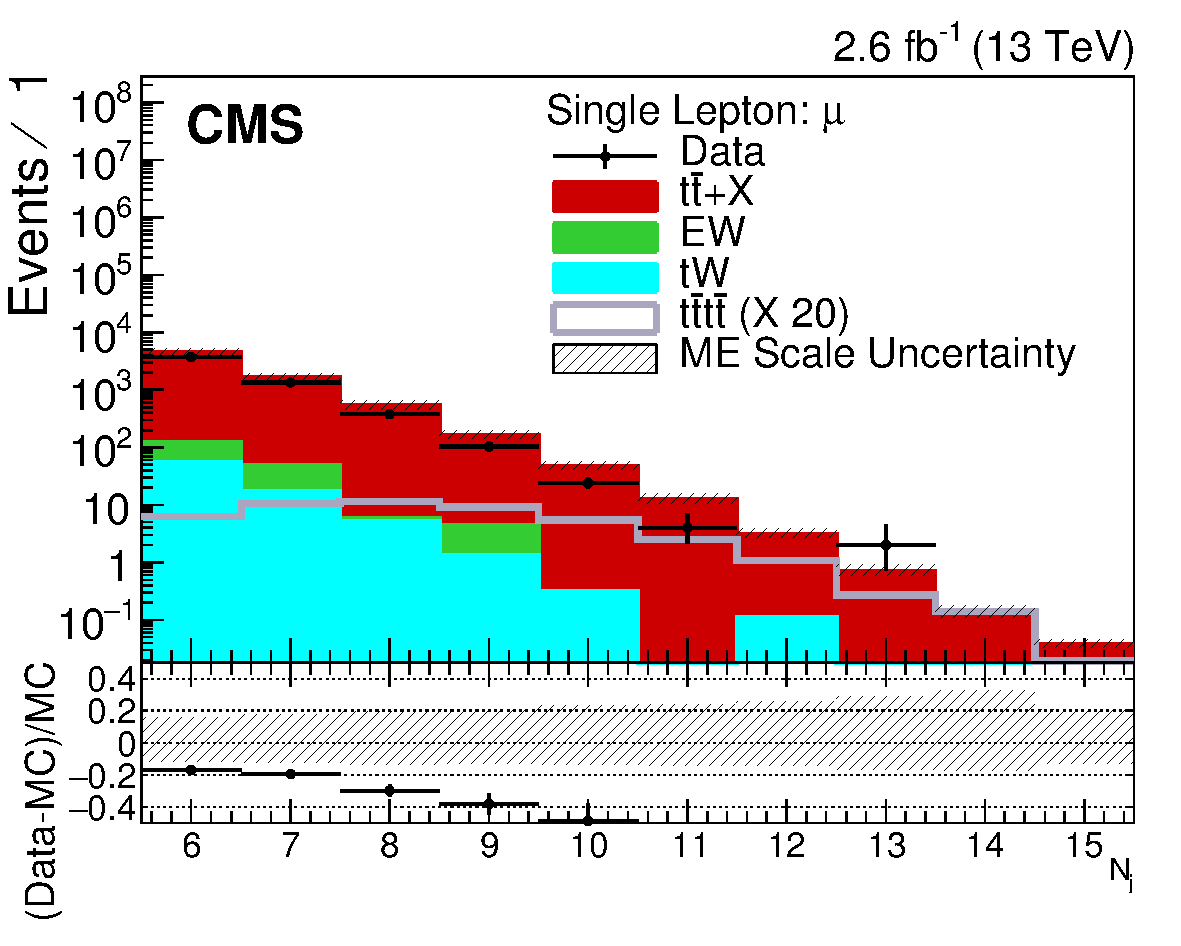
\includegraphics[width=0.48\textwidth]{images/Run2/nJets_StackLogY_woAlphaS.pdf}
    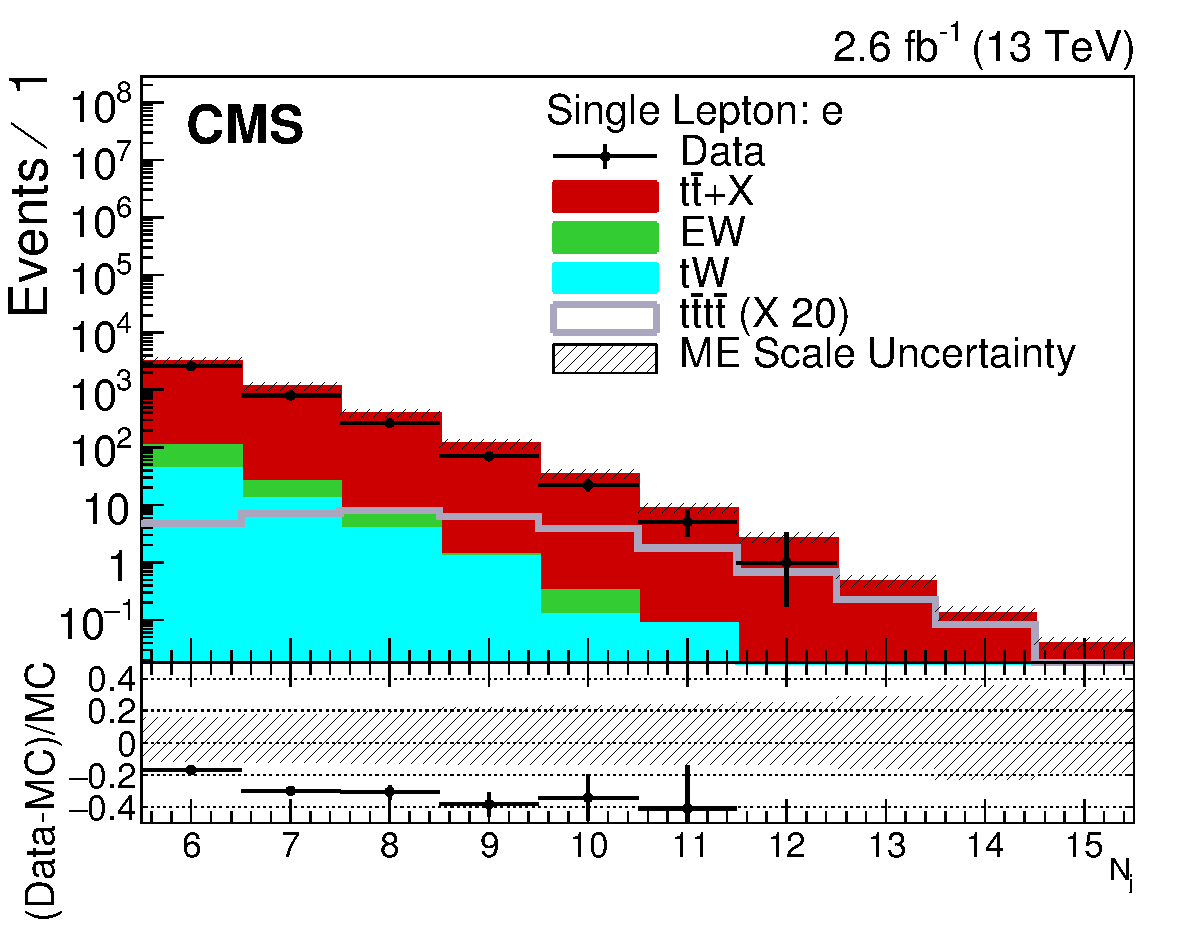
\includegraphics[width=0.48\textwidth]{images/Run2/nJets_StackLogY_e_woAlphaS.pdf}
    \caption{The \njets distributions for data and simulation in the $\mu$ + jets channel (left) and $e$ + jets channel (left) without jet multiplicity modelling scale factors applied.}
    \label{fig:withoutAlpha}
\end{figure}

The scale factors applied for the heavy flavour modelling are described in Section~\ref{ttbbmod}. The distributions for the \nMtags are shown with and without the heavy flavour modelling scale factors applied. It is not obvious that there is a significant improvement in the \nMtags after the scale factors have been applied but the heavy flavour fraction is allowed to float as a shape nuisance parameter in the template fit.

\begin{figure}[ht!]
    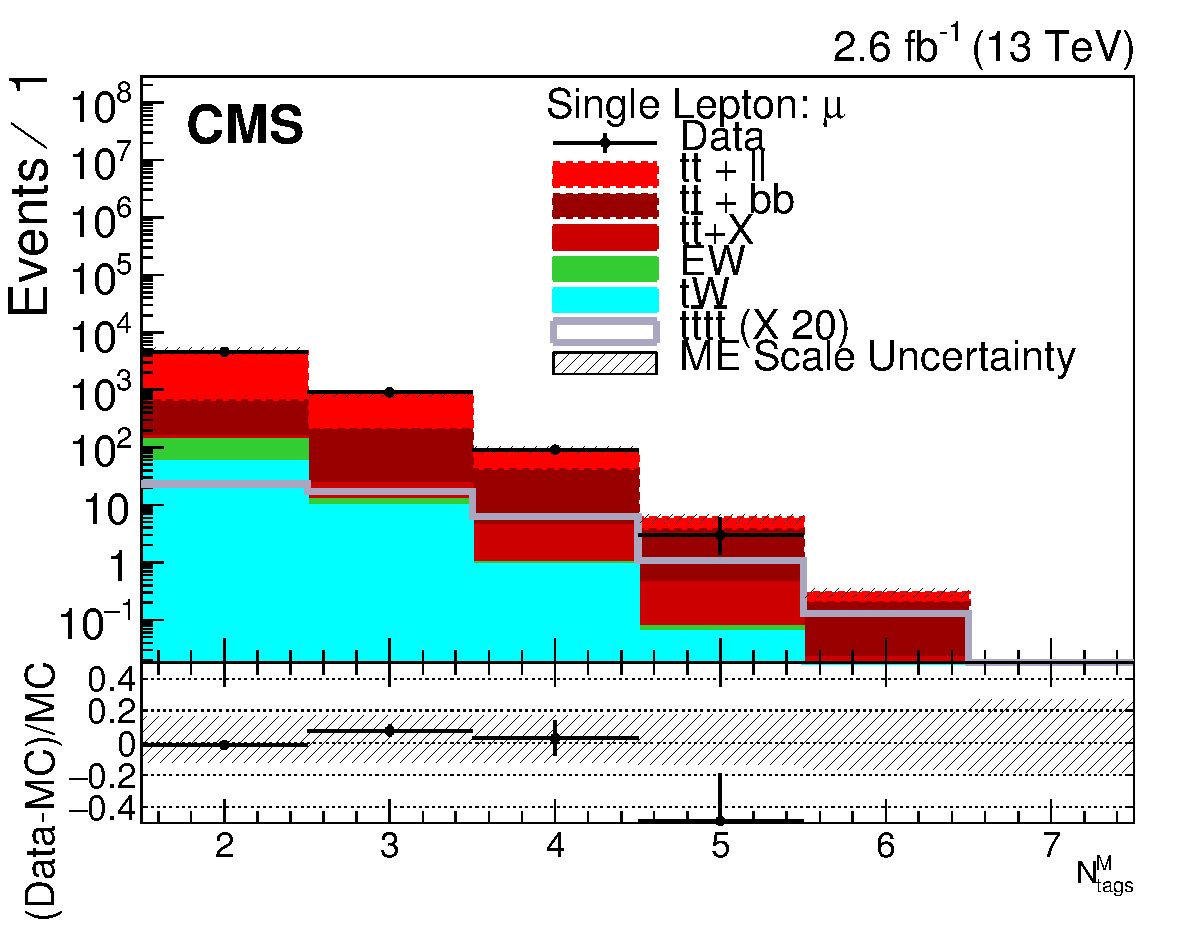
\includegraphics[width=0.47\textwidth]{images/Run2/nMtags_StackLogY_HF_wo_reweight.pdf} 
    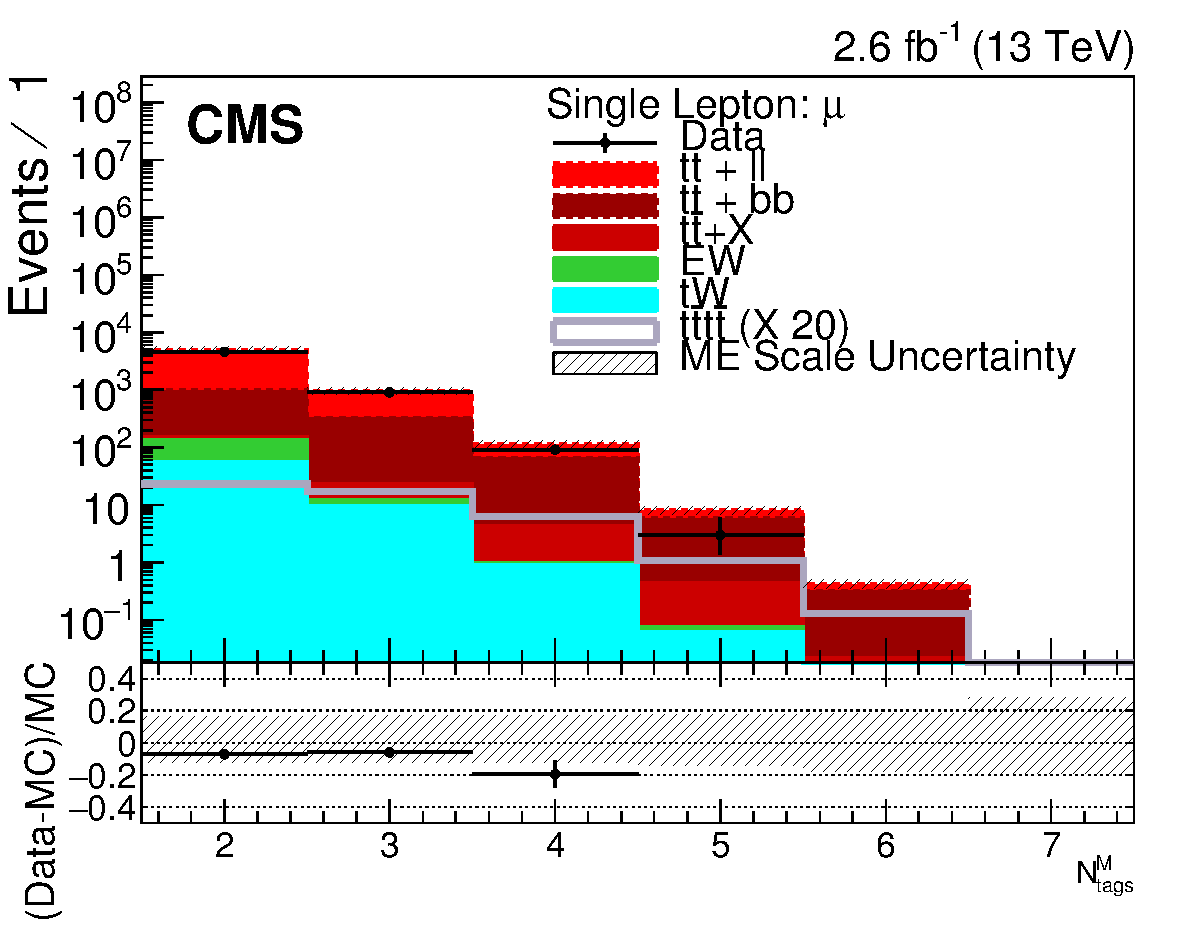
\includegraphics[width=0.47\textwidth]{images/Run2/nMtags_StackLogY_HF_w_reweight.pdf} 
    \caption{\nMtags are shown for the muon channel with heavy flavour reweighting (right) and without(left).}
    \label{fig:HF_reweight}
\end{figure}

\section{Weighted event counts at each baseline event selection requirement \label{cutflow13}}

\section{Data-simulation agreement}

\section{Discriminating between signal and background}
\label{sec:discriminating13}

It can be seen in Section~\ref{cutflow13} that the \ttbar background is three orders of magnitude larger in the signal region. The variables used to discriminate between \ttbar and \tttt are described below.
% There are three main features which can be used to discriminate; the number of top quarks which can be reconstructed in the event, the number of b-jets found in each event, and event activity such as \HT.

\subsection{Hadronic top quark content}
\label{sec:topContent13}

As the \antikt algorithm cannot resolve jets which have $\Delta R = \sqrt{  \theta^{2} + \phi^{2} } < 0.4$, a hadronically decaying top quark can only be deemed \emph{reconstructible} if the minimal $\Delta R$ between all three jets is $> 0.4$ which happens $> 98\%$ of the time in \ttbar and \tttt simulation when studying the decay products of leptons and partons, and pairs of partons.\\
The BDT training was performed on 273~K \ttbar events. The input variables to the hadronic top quark reconstruction BDT are shown in Fig.~\ref{fig:TrijetBDTInputFeatures13}. The separation power for each of these variables and for the output BDT discriminator distribution in Fig.~\ref{fig:TrijetBDTOutput13} is evident as in the \runone chapter. 

\begin{figure}[ht!]
\centering
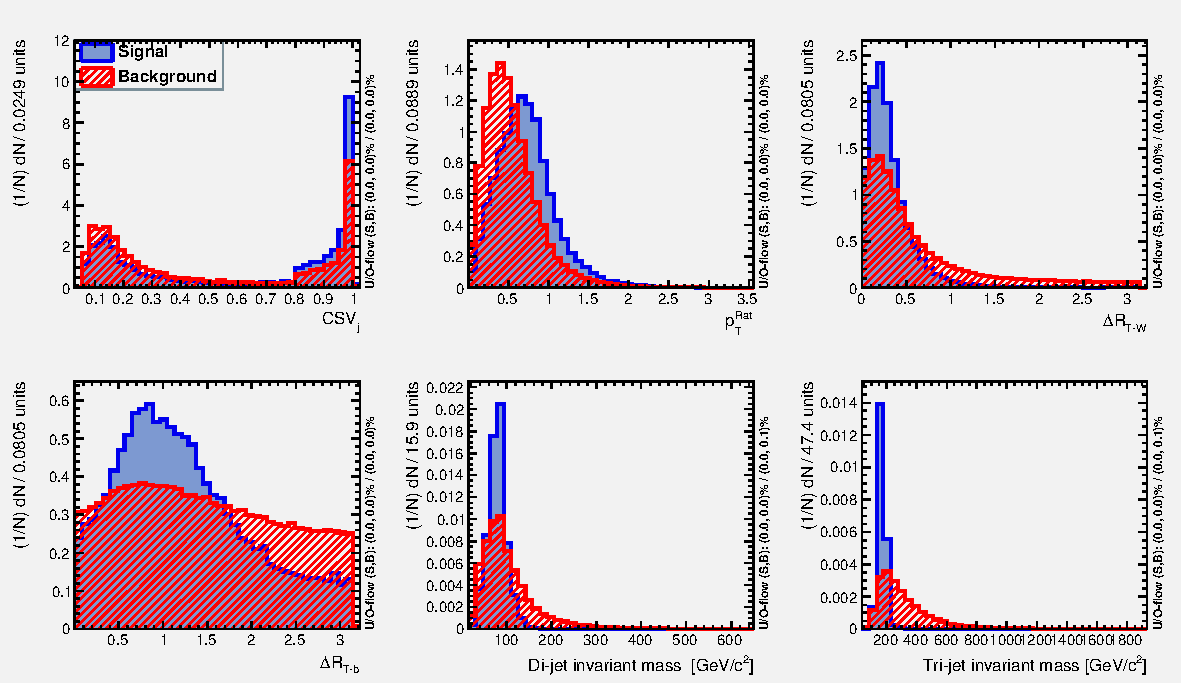
\includegraphics[width=\linewidth]{images/Run2/variables_id_c1.pdf}
\caption{Normalised distributions of the six variables used the MVA hadronic Top kinematic reconstruction are shown for good (red histograms) and bad (blue histograms) trijets.}
\label{fig:TrijetBDTInputFeatures13}
\end{figure}

\begin{figure}[ht!]
\begin{center}
    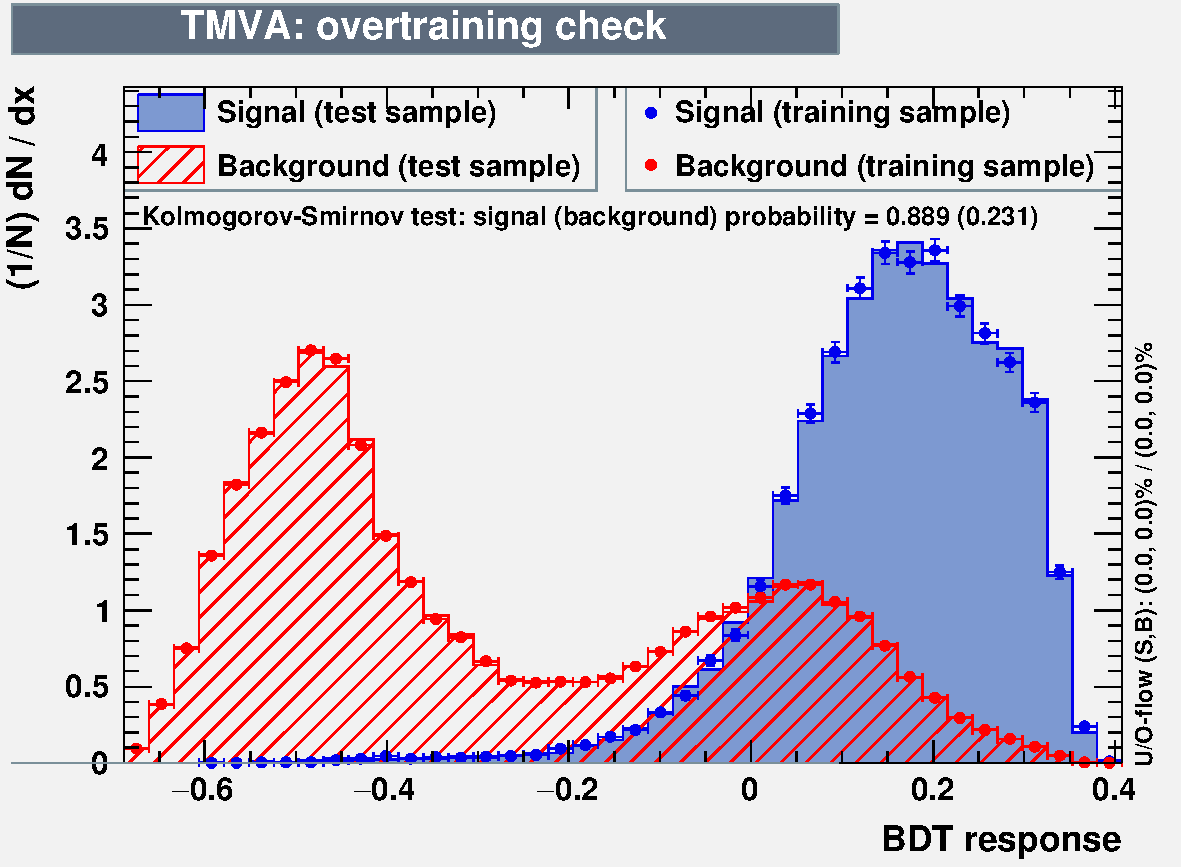
\includegraphics[width=0.55\textwidth]{images/Run2/overtrain_BDT.pdf}
    \caption{The discriminator distributions for the BDT classifier for good and bad trijets in training and validation samples.}
    \label{fig:TrijetBDTOutput13}
\end{center}
\end{figure}

The affect of the tri-jet invariant mass variable in the BDT is shown in Fig.~\ref{fig:multimode13} where it can be clearly seen that this variable contributes to the strong splitting of the BDT output distribution at a value of $\approx-0.2$.

\begin{figure}[ht!]
\begin{center}
    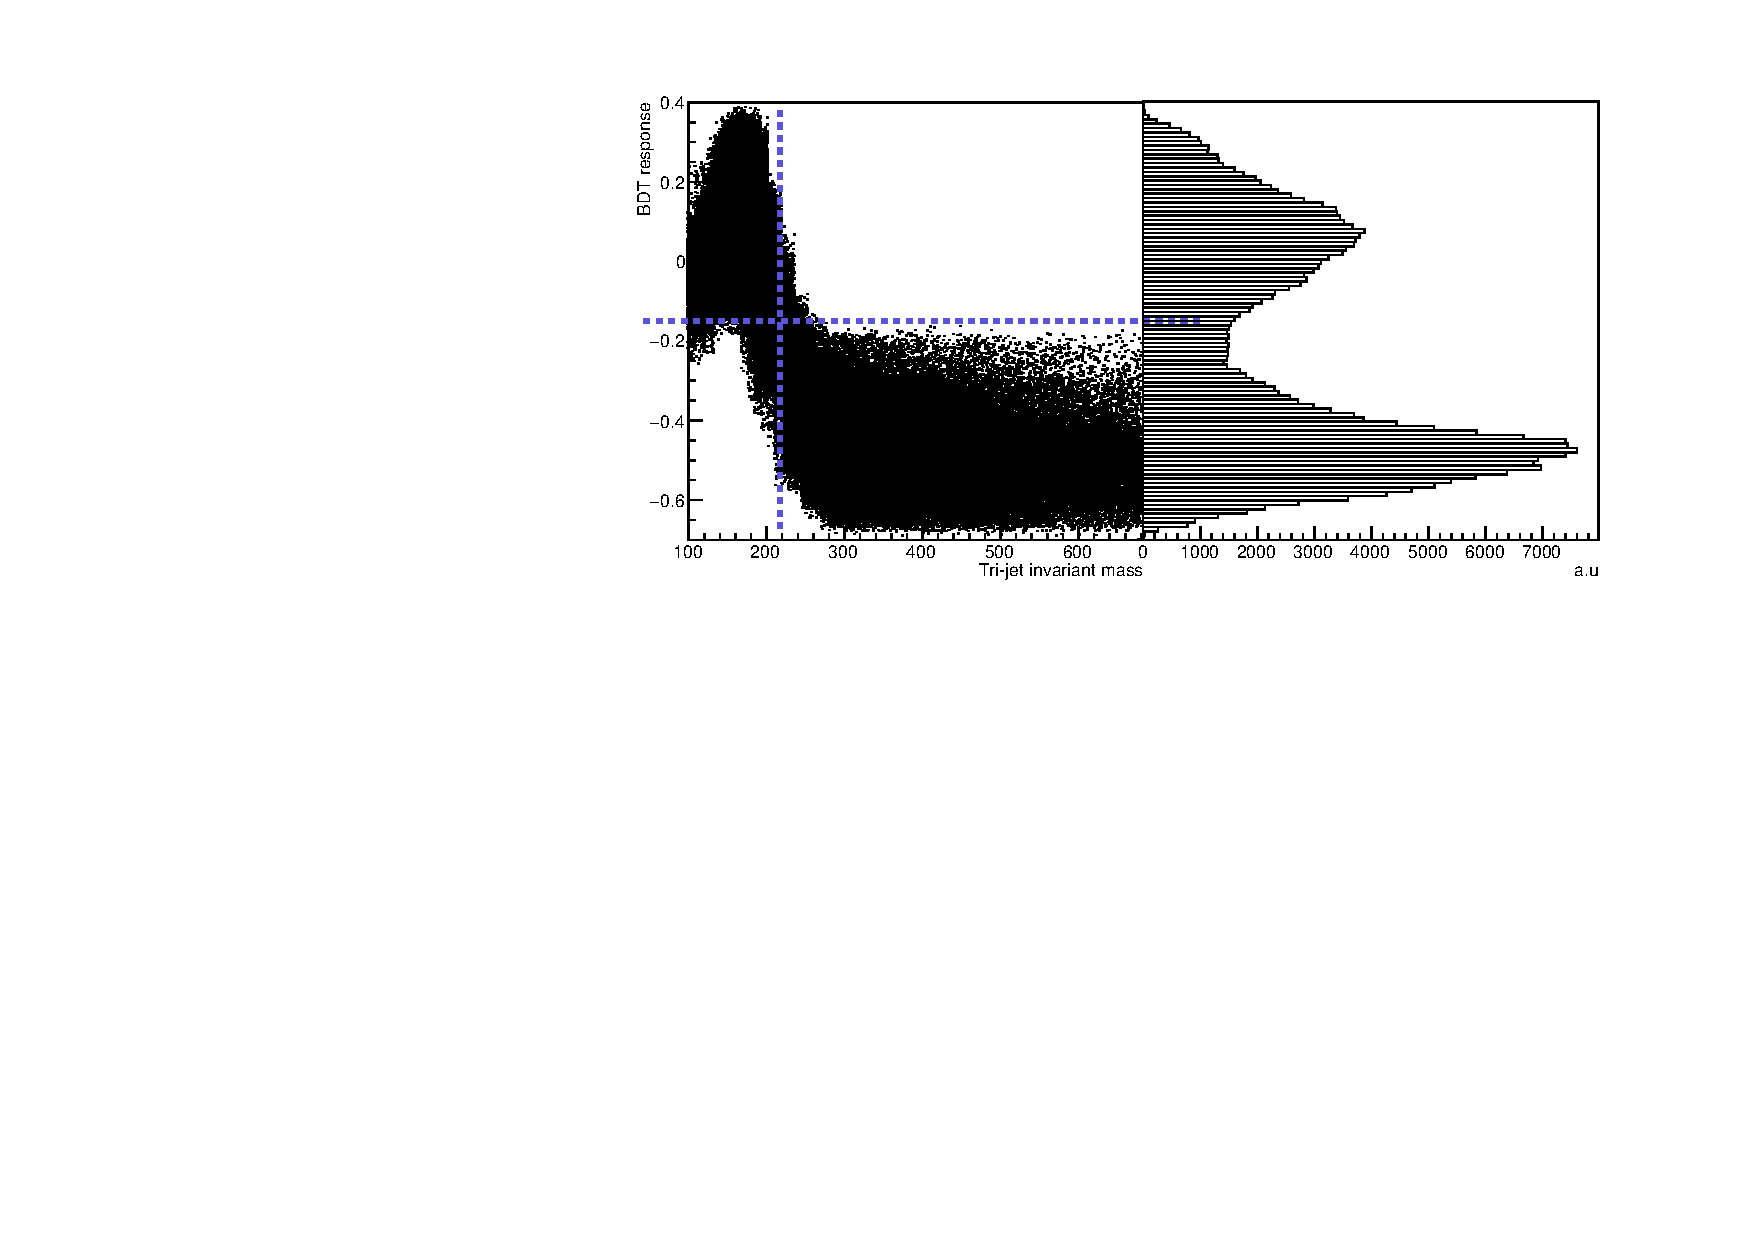
\includegraphics[width=0.85\textwidth]{images/Run2/multimode.pdf}
    \caption{The discriminator distributions for the BDT classifier versus trijet invariant mass and the projection on the vertical axis. Dashed lines indicate the cut value on trijet invariant mass at the BDT root node.}
    \label{fig:multimode13}
\end{center}
\end{figure}

In Fig.~\ref{fig:ContoursTopMassHadrWmass13}, the left-hand plot shows the distribution of good and bad tri-jet combinations in the phase space of tri-jet and di-jet invariant mass. It can be seen from the right-hand plot in Fig.~\ref{fig:ContoursTopMassHadrWmass13} that high BDT discriminator values are found in the region where the good tri-jet combinations are clustered.
\begin{figure}[ht!]
\begin{center}
    \includegraphics[width=\textwidth]{images/Run2/ContoursHadrWmassTopMass.pdf}
    \caption{(Left)  Di-jet versus trijet invariant mass distribution for good (blue) and bad (red) trijet combinations. (Right) The average BDT response as a function of Di-jet versus trijet invariant mass input variables.}
    \label{fig:ContoursTopMassHadrWmass13}
\end{center}
\end{figure}

\subsubsection*{BDT$_{tri-jet2}$}

The distribution for BDT$_{tri-jet2}$ is shown in Fig.~\ref{fig:bdtTrijet213}. There is good agreement between the data and simulation and sufficient discrimination power to be used in the event-level BDT.

\begin{figure}[ht!]
    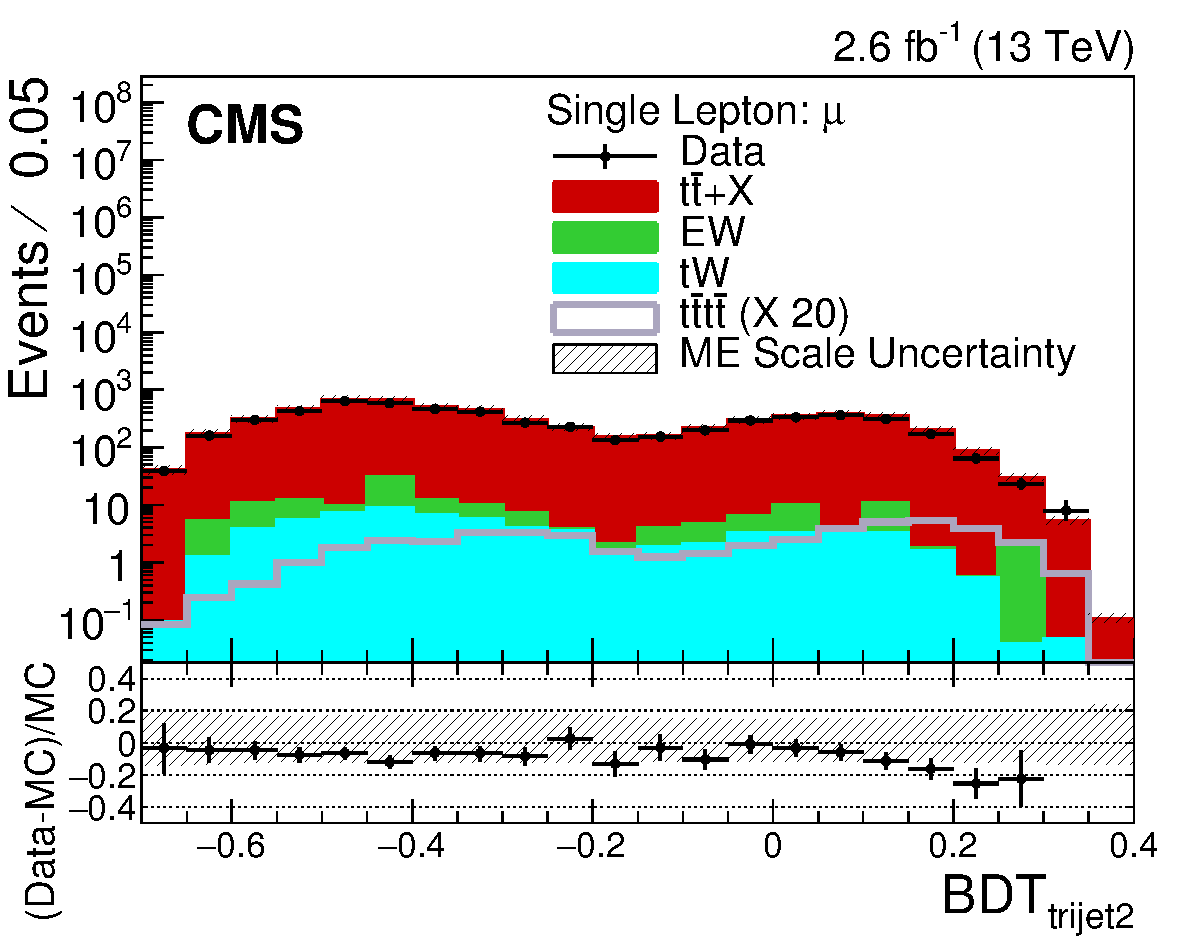
\includegraphics[width=0.44\textwidth]{images/Run2/BDT_trijet2_StackLogY.pdf}
    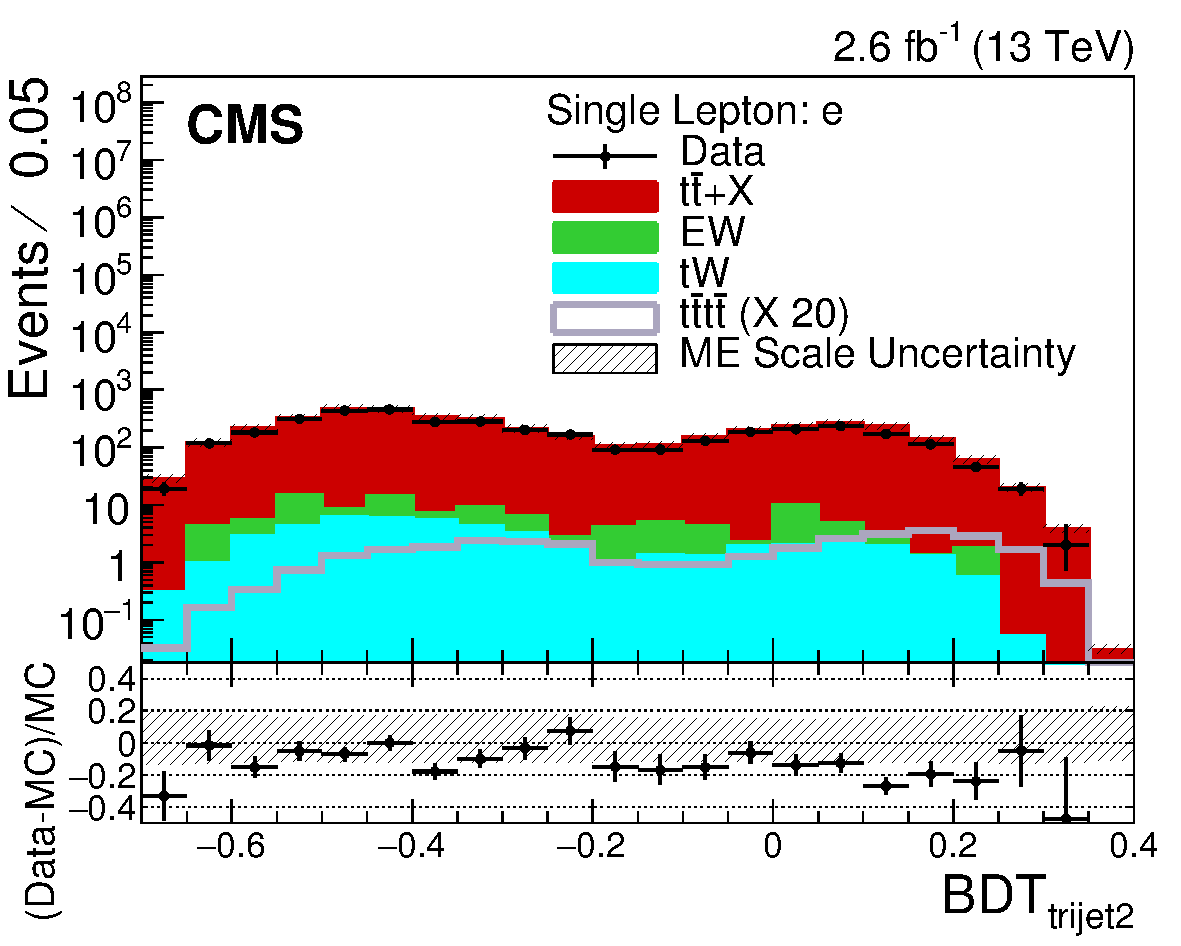
\includegraphics[width=0.44\textwidth]{images/Run2/BDT_trijet2_StackLogY_e.pdf}
    \caption{ The BDT$_{trijet2}$ distributions for data and simulation event in the $\mu$ + jets channel (left) and $e$ + jets channel (right) are plotted.}
    \label{fig:bdtTrijet213}
\end{figure}

\subsubsection*{Reduced Event Variables}

The reduced variables formed from the reduced event, where the jets from the highest-ranked hadronic top quark have been removed from the collection of jets, are shown in Figs.~\ref{fig:htx13} and~\ref{fig:sumjetmassx13}. Again, good agreement is observed between the data and simulation and both variables were found to have good discrimination power in the event-level BDT.

\begin{figure}[ht!]
    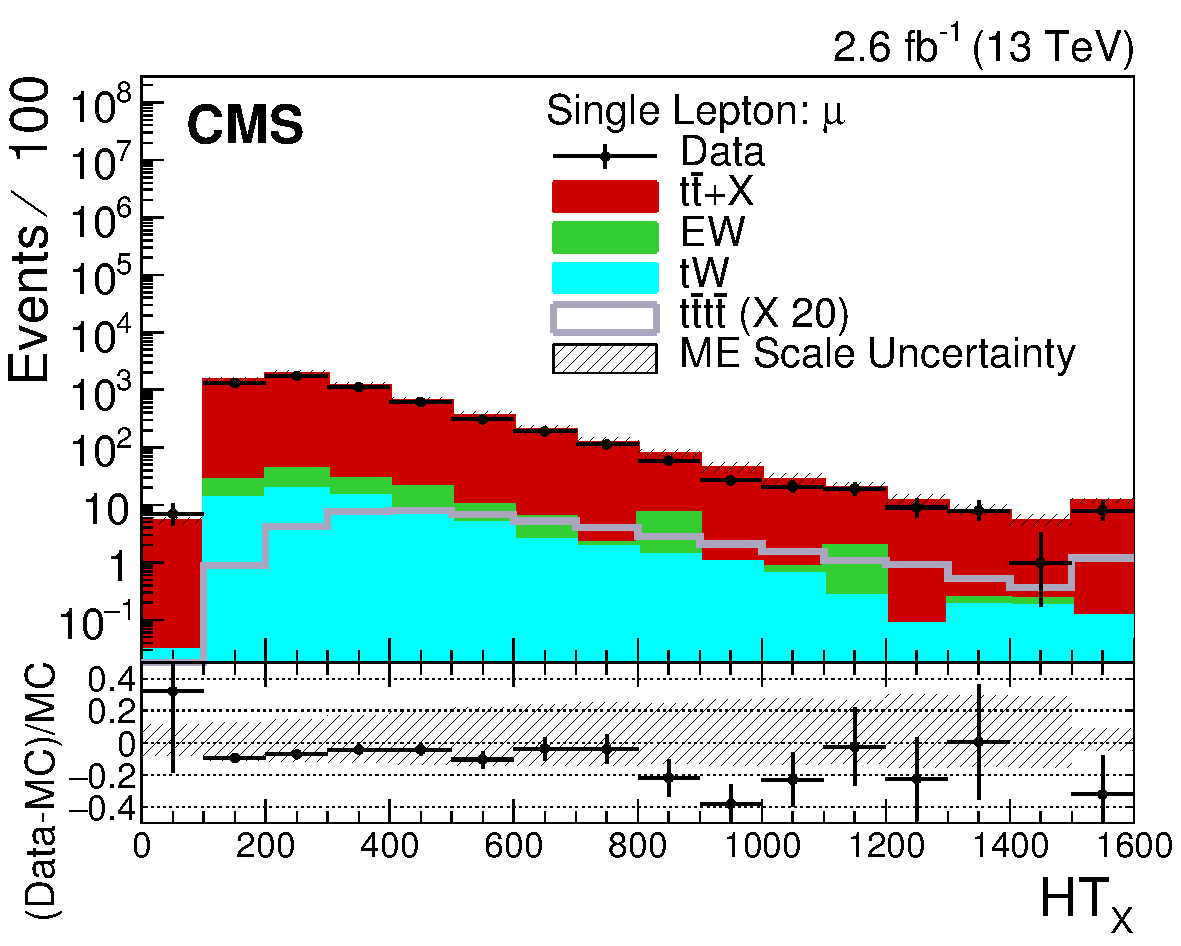
\includegraphics[width=0.44\textwidth]{images/Run2/HTX_StackLogY.pdf}
    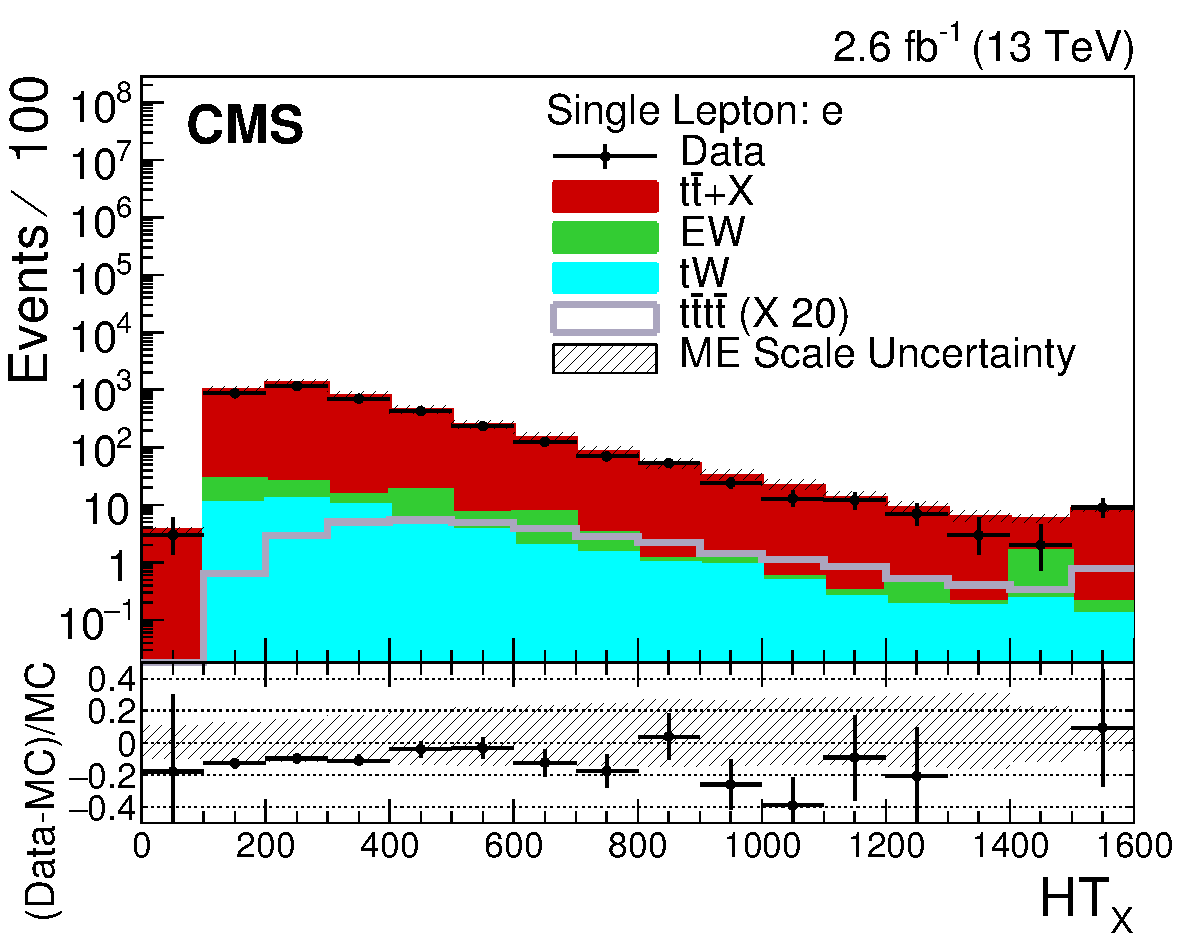
\includegraphics[width=0.44\textwidth]{images/Run2/HTX_StackLogY_e.pdf}
    \caption{ The \HTX distributions for data and simulation event in the $\mu$ + jets channel (left) and $e$ + jets channel (right) are plotted.}
    \label{fig:htx13}
\end{figure}

\begin{figure}[ht!]
    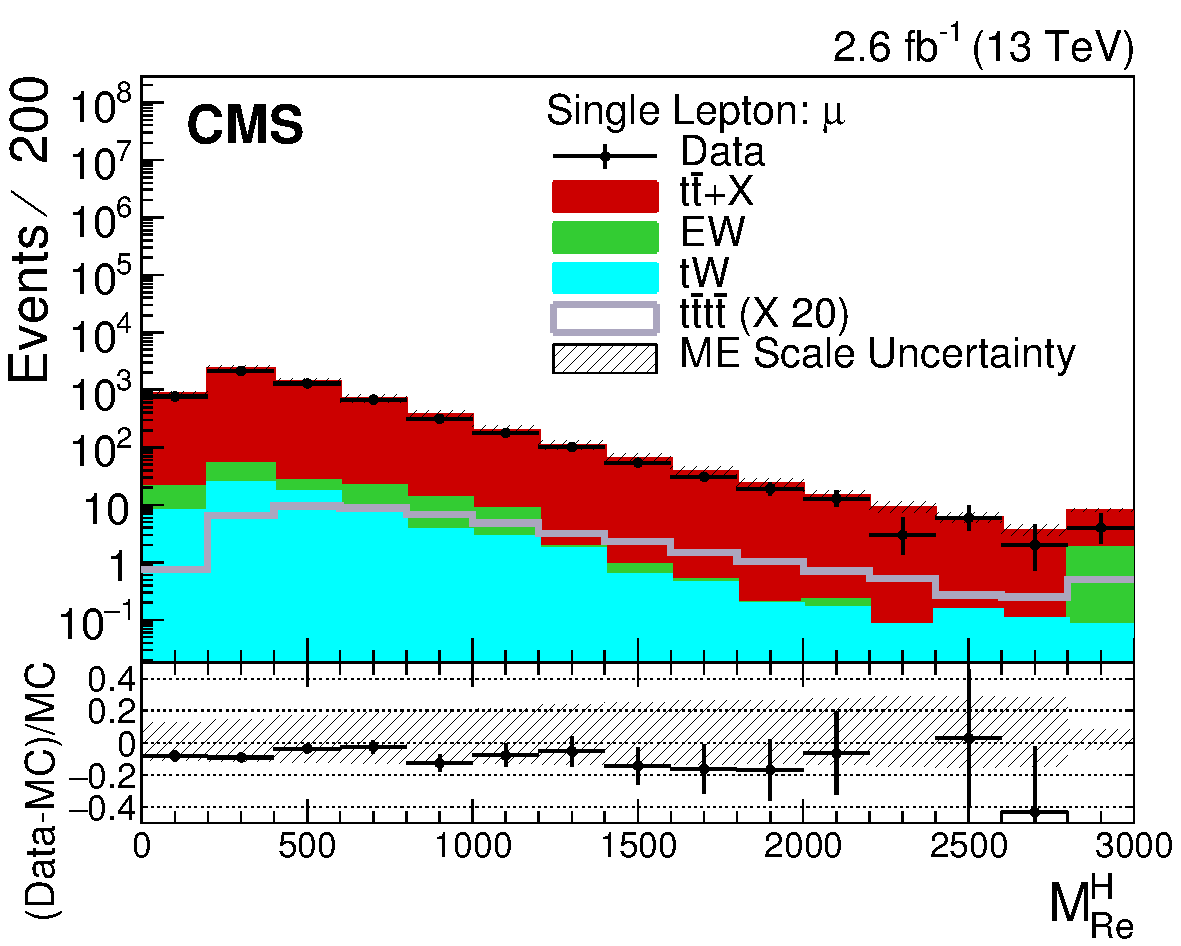
\includegraphics[width=0.44\textwidth]{images/Run2/SumJetMassX_StackLogY.pdf}
    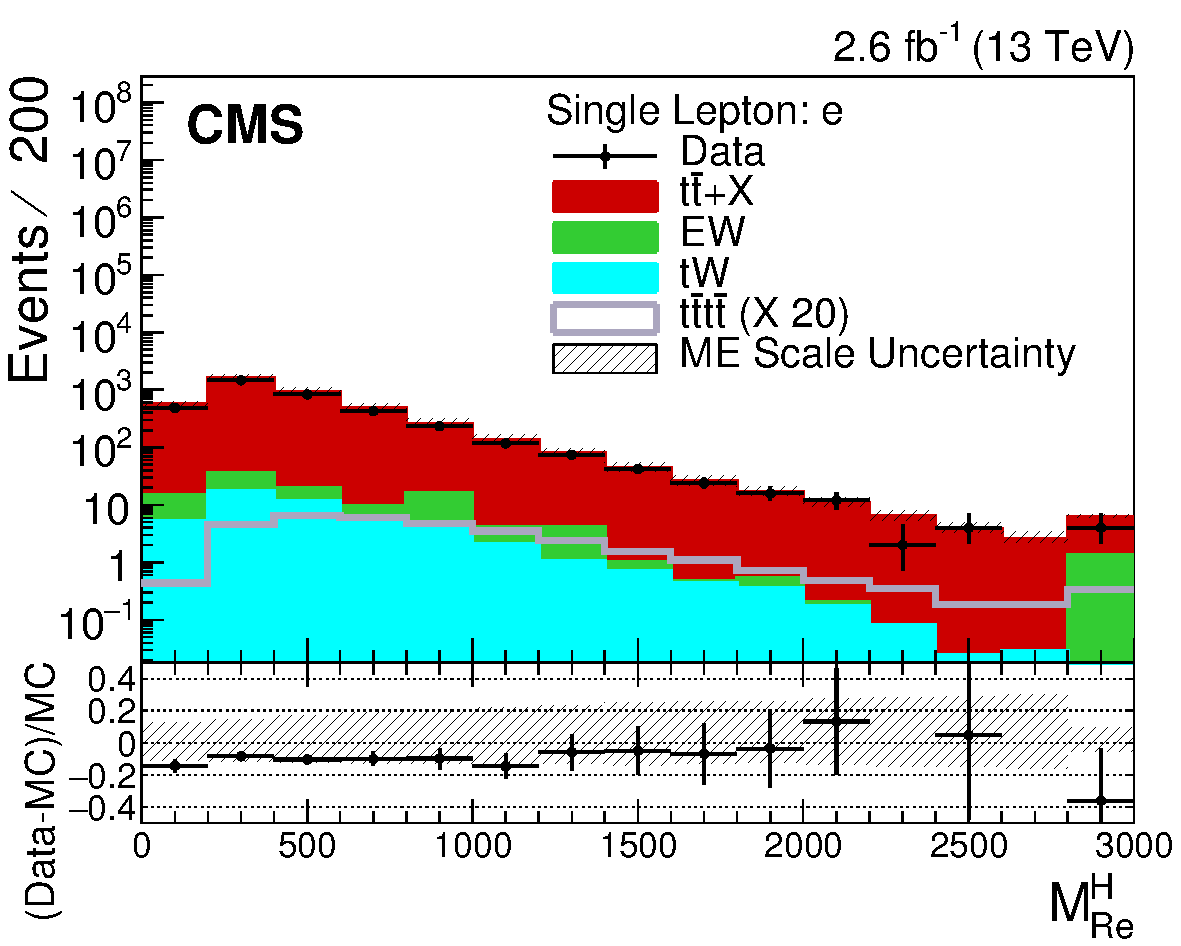
\includegraphics[width=0.44\textwidth]{images/Run2/SumJetMassX_StackLogY_e.pdf}
    \caption{ The \redhadmass distributions for data and simulation event in the $\mu$ + jets channel (left) and $e$ + jets channel (right) are plotted.}
    \label{fig:sumjetmassx13}
\end{figure}


\subsection{Event activity and b-jet content variables chosen for the event-level BDT}

The following variables were chosen for their discrimination power within the event-level BDT and are previously described in section~\ref{sec:Strategy}. It should be noted that the third-highest CSV and fourth-highest CSV values can be used in the $\sqrt{s} = 13$~TeV analysis as the CSV distributions have been corrected by the modelling in section~\ref{subsec:method2btag}.


\begin{multicols}{2}
\setlength{\columnseprule}{0pt} 

\begin{itemize}
\item \htb
\item \htrat
\item \njets
\item lepton \pt, \leadleppt
\item \njetsw
\item third-highest CSV
\item fourth-highest CSV
\end{itemize}

\end{multicols}

\subsection{Event-level BDT}


\section{Systematic uncertainties}
\label{sec:uncertainties13}

\section{Template fit and upper limit}
\label{sec:limit13}

\section{Systematics studies and tests on analysis}


\section{Summary and conclusion}
\label{sec:summary13}

\section{Discussion of ATLAS four-top-quark production studies at $\sqrt{s} =$~13~TeV}
\label{sec:ATLASresult13}
% \fxnote{Possible comparison with atlas requirements put into our framework}
